\section{NVTrust Chain-Binding}
\label{sec:nvtrust}

\subsection{Double-Spend Prevention}

The fundamental security challenge in multi-chain AI mining is preventing ``copy-paste mining''---submitting the same work to multiple chains for multiple rewards. PoAI solves this via \textbf{chain-binding}: cryptographically committing each unit of work to a specific chain before computation begins.

\begin{definition}[Double-Spend Attack]
An attacker performs work $W$ once but claims rewards on chains $C_1, C_2, \ldots, C_n$ by submitting the same or slightly modified proofs.
\end{definition}

\begin{theorem}[Double-Spend Resistance]
Under chain-binding with NVTrust attestation, the probability of a successful double-spend is:
\begin{equation}
P(\text{double-spend}) \leq \text{negl}(\lambda)
\end{equation}
where $\lambda$ is the security parameter (256-bit for BLAKE3).
\end{theorem}

\subsection{Work Context Structure}

Before any computation begins, the miner commits to a \textbf{WorkContext}:

\begin{lstlisting}[style=rust]
pub struct WorkContext {
    pub chain_id: u64,           // Target chain: 36963/200200/96369
    pub job_id: [u8; 32],        // Unique job identifier
    pub model_hash: [u8; 32],    // BLAKE3(model_weights)
    pub input_hash: [u8; 32],    // BLAKE3(input_data)
    pub device_id: [u8; 32],     // GPU hardware identifier
    pub nonce: [u8; 32],         // Fresh randomness
    pub timestamp: u64,          // Unix timestamp
}
\end{lstlisting}

\subsection{NVTrust Attestation Flow}

\begin{enumerate}
    \item \textbf{Pre-Compute Commitment}: Miner creates WorkContext with target chain ID
    \item \textbf{TEE Initialization}: Context passed to NVTrust enclave
    \item \textbf{Secure Execution}: AI workload runs inside GPU TEE
    \item \textbf{Receipt Generation}: Enclave creates attested receipt
    \item \textbf{Hardware Signature}: NVTrust signs receipt with device key
    \item \textbf{Chain Submission}: Receipt submitted to committed chain
\end{enumerate}

\begin{center}
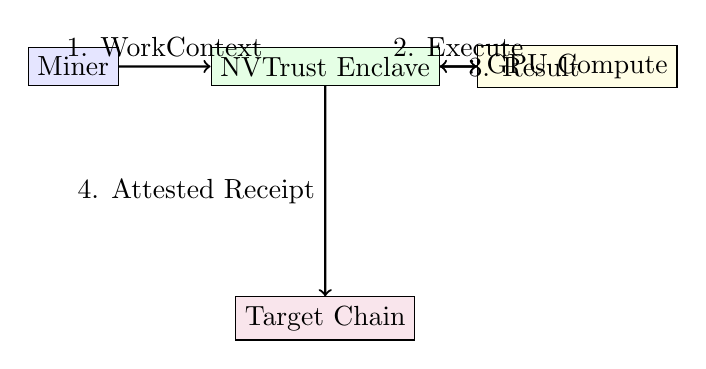
\begin{tikzpicture}[scale=0.8]
    \node[draw, rectangle, fill=blue!10] (miner) at (0,4) {Miner};
    \node[draw, rectangle, fill=green!10] (nvtrust) at (4,4) {NVTrust Enclave};
    \node[draw, rectangle, fill=yellow!10] (gpu) at (8,4) {GPU Compute};
    \node[draw, rectangle, fill=purple!10] (chain) at (4,0) {Target Chain};

    \draw[->, thick] (miner) -- node[above] {1. WorkContext} (nvtrust);
    \draw[->, thick] (nvtrust) -- node[above] {2. Execute} (gpu);
    \draw[->, thick] (gpu) -- node[right] {3. Result} (nvtrust);
    \draw[->, thick] (nvtrust) -- node[left] {4. Attested Receipt} (chain);
\end{tikzpicture}
\end{center}

\subsection{Attested Receipt}

The NVTrust enclave produces an \textbf{AttestedReceipt}:

\begin{lstlisting}[style=rust]
pub struct AttestedReceipt {
    pub context: WorkContext,         // Original commitment
    pub result_hash: [u8; 32],        // BLAKE3(output)
    pub work_metrics: WorkMetrics,    // FLOPs, tokens, time
    pub nvtrust_signature: Vec<u8>,   // GPU hardware signature
    pub spdm_evidence: SPDMEvidence,  // Firmware measurements
}

pub struct SPDMEvidence {
    pub version: u8,
    pub measurement_hash: [u8; 48],   // GPU firmware hash
    pub nonce: [u8; 32],              // Replay protection
    pub signature: Vec<u8>,           // SPDM signature
    pub certificate_chain: Vec<u8>,   // Chain to NVIDIA root
}
\end{lstlisting}

\subsection{Spent Set}

Each chain maintains a \textbf{SpentSet} to track minted work:

\begin{definition}[Work ID]
The unique identifier for a unit of work is:
\begin{equation}
\text{work\_id} = \text{BLAKE3}(\text{device\_id} \| \text{nonce} \| \text{chain\_id})
\end{equation}
\end{definition}

\begin{property}[Spent Set Invariant]
For all valid blocks $B$ and proofs $P \in B$:
\begin{equation}
\text{work\_id}(P) \notin \text{SpentSet}(B.\text{prev}) \land \text{work\_id}(P) \in \text{SpentSet}(B)
\end{equation}
\end{property}

\begin{algorithm}
\caption{CheckAndMarkSpent}
\begin{algorithmic}[1]
\Require AttestedReceipt $R$, SpentSet $S$
\Ensure Boolean (success), SpentSet (updated)
\State $\text{work\_id} \gets \text{BLAKE3}(R.\text{context}.\text{device\_id} \| R.\text{context}.\text{nonce} \| R.\text{context}.\text{chain\_id})$
\If{$\text{work\_id} \in S$}
    \State \Return (\textbf{false}, $S$) \Comment{Already minted}
\EndIf
\State $S' \gets S \cup \{\text{work\_id}\}$
\State \Return (\textbf{true}, $S'$)
\end{algorithmic}
\end{algorithm}

\subsection{Chain ID Validation}

Before processing any receipt, validators check chain binding:

\begin{lstlisting}[style=rust]
fn validate_chain_binding(
    receipt: &AttestedReceipt,
    expected_chain_id: u64,
) -> Result<(), MiningError> {
    if receipt.context.chain_id != expected_chain_id {
        return Err(MiningError::WrongChain {
            expected: expected_chain_id,
            got: receipt.context.chain_id,
        });
    }
    Ok(())
}
\end{lstlisting}

\subsection{Multi-Chain Mining}

The same GPU can mine for multiple chains, but requires \textbf{separate work} for each:

\begin{center}
\begin{tabular}{lccc}
\toprule
\textbf{GPU} & \textbf{Hanzo (36963)} & \textbf{Zoo (200200)} & \textbf{Lux (96369)} \\
\midrule
H100-001 & nonce: 0x1a... & nonce: 0x2b... & nonce: 0x3c... \\
H100-001 & Receipt A & Receipt B & Receipt C \\
H100-001 & \checkmark Valid & \checkmark Valid & \checkmark Valid \\
\bottomrule
\end{tabular}
\end{center}

\begin{lemma}[Cross-Chain Independence]
Receipts $R_A$ and $R_B$ with different chain IDs are independent:
\begin{equation}
\text{work\_id}(R_A) \neq \text{work\_id}(R_B) \iff R_A.\text{chain\_id} \neq R_B.\text{chain\_id}
\end{equation}
\end{lemma}

\subsection{Supported GPU Hardware}

\begin{center}
\begin{tabular}{lccc}
\toprule
\textbf{GPU Model} & \textbf{CC Support} & \textbf{Trust Score} & \textbf{Reward Multiplier} \\
\midrule
GB200 & Full NVTrust + TEE-I/O & 100 & 1.5x \\
B200 & Full NVTrust + TEE-I/O & 100 & 1.5x \\
B100 & Full NVTrust + TEE-I/O & 100 & 1.5x \\
H200 & Full NVTrust & 95 & 1.3x \\
H100 & Full NVTrust & 95 & 1.3x \\
RTX PRO 6000 & NVTrust & 85 & 1.1x \\
RTX 5090 & Software only & 60 & 0.8x \\
RTX 4090 & Software only & 60 & 0.8x \\
\bottomrule
\end{tabular}
\end{center}

\textbf{Key Invariant:} The same AI work cannot be minted on Hanzo, Lux, AND Zoo---only on the chain specified in the pre-committed WorkContext.chain\_id.
